\documentclass{article} % 单栏排版
% 中文支持
\usepackage[UTF8]{ctex}            % 支持中文
\usepackage{amsmath, amssymb, amsthm}      % 数学符号与公式
\usepackage{graphicx}              % 插入图片
\usepackage{caption}               % 图表标题
\usepackage{float}                 % 图表位置控制
\usepackage{geometry}              % 页面设置
\usepackage{fancyhdr}              % 页眉页脚
\usepackage{abstract}              % 摘要环境优化
\usepackage{indentfirst}           % 首段缩进
\usepackage{setspace}              % 行距设置
\usepackage{hyperref}              % 超链接
\usepackage{dutchcal}
\usepackage{bm}
\usepackage{fmtcount}
\usepackage{mathtools}
\usepackage{booktabs}
\usepackage{array}
\usepackage{tikz}
\usepackage[european resistors]{circuitikz}
\usepackage{siunitx}
\usepackage{subcaption}
\usepackage{pgfplots}
\usepackage{fix-cm}
\usepackage{mathrsfs}
\pgfplotsset{compat=1.18}
\newcommand{\di}{\mathrm{d}}
\newcommand{\ii}{\mathrm{i}}
\newcommand{\e}[1]{\mathrm{e}^{#1}}
\newcommand{\f}[1]{\mathscr{F}\left[#1\right]}
\newcommand{\fo}[1]{\mathscr{F}^{-1}\left[#1\right]}
\DeclareMathOperator{\sgn}{sgn}
\ctikzset{
    bipoles/length = 1cm,
    resistors/scale = 0.8,
    capacitors/scale = 0.8,
}
% 页面设置（单栏，适合长篇推导）
\geometry{
  a4paper,
  left=2.0cm,
  right=2.0cm,
  top=2.5cm,
  bottom=2.5cm,
}
% 行距
\setstretch{1.5}
% 标题格式
\title{\LARGE \bfseries 离散Fourier变换下网格电路的阻抗奇异性与拓扑输运}
\author{
  PB25050895\ 朱克拉$^{1}$，\quad PB25050892\ 王思晗$^{1}$ \\
  \small (1.中国科学技术大学工程科学学院，合肥)
}
\date{}
% 重定义摘要环境
\renewenvironment{abstract}{\small
  \textbf{摘\ \ 要：}
}{}
\newenvironment{keyword}{\small
  \textbf{关键词：}  
}{}
% 首行缩进
\setlength{\parindent}{2em}
% 图表标题格式
\captionsetup[figure]{labelformat=default, labelsep=quad, font=small}
\captionsetup[table]{labelformat=default, labelsep=quad, font=small}
% 英文摘要
\newenvironment{abstract_en}{%
  \small
  \textbf{Abstract:}%
}{%
  \par
}
% 英文关键词
\newenvironment{keyword_en}{\small
  \textbf{Keywords:}  
}{}



\begin{document}

\maketitle

\begin{abstract}
  本文针对二维网格纯电阻和一维$LC$拓扑电路在谐振下的行为，前者使用离散Fourier变换方法，将基尔霍
  夫定律转化为频域代数方程。推导出任意两点间等效电阻的积分表达式，并进一步通过留数定理和级数展开，
  得到了适用于数值计算的级数求和公式
  研究了二维无穷$LC$网格中的电学性质，尤其对$\omega^2LC = 1$下的特殊阻抗行为进行了分析计算。
  系统分析了两种二维无穷网格电路的输运性质。本文的推导过程完整、严谨，可为相关领域的理论分析
  和教学参考提供有益借鉴。
\end{abstract}

\begin{keyword}
  离散Fourier变换；网格电阻；SSH电路；阻抗积分；$LC$网络
\end{keyword}

\vspace*{1em}

\begin{abstract_en}
Using discrete Fourier transform as a unified tool, 
we investigate transport in two-dimensional infinite
 grid circuits. For resistive networks, we derive an 
 integral expression for the equivalent resistance and
  convert it to a rapidly convergent series via residue
   calculus. For $LC$ networks at the critical frequency
    $\omega^2 LC = 1$, we find that the impedance vanishes
     when the two nodes have the same parity, and becomes a 
     constant purely imaginary value otherwise, revealing an
      alternating pattern of perfect transmission and complete
       blockade. All analytical results are confirmed by numeric
       al Cauchy principal value integrations.
\end{abstract_en}

\begin{keyword_en}
  discrete Fourier transform; grid resistance; SSH circuit; impedance integration; $LC$ network
\end{keyword_en}


\vspace*{1em}



\section{引言}

二维无穷网格电路的输运性质是凝聚态物理、电路理论与工程应用中的重要问题。
电阻网格的等效电阻计算不仅是电学中的经典问题，其在网络分析
和数值算法中亦有重要应用。与此同时，由电容和电感构成的$LC$网格则展现了
更为丰富的频率响应特性，与离散微波、超材料密切相关。

离散Fourier变换（Discrete Fourier Transform, DFT）是处理此类离散平移对称
系统的有力工具。通过将实空间中的差分方程变换至频域，可将复杂的求和或积分
问题转化为代数运算，再通过逆变换还原物理量。本文从纯电阻网格入手，
通过展示DFT在纯电阻网格中的性质，从而以相似的方式迁移运用到LC网格中。
其中还介绍了$LC$电路构造想法的由来——一维SSH电路，受到其中阻抗为0时电路
奇异性质的启发，本文探究了其$Z(\omega)=0$的特殊情况，发现横纵坐标奇偶性相同的点
与原点之间的阻抗均为0，其余点阻抗均为定值的现象，并对其展开进一步研究。


\section{纯电阻网格的Fourier分析}

\subsection{问题背景与基尔霍夫方程}

\begin{figure}[H]
  \centering
  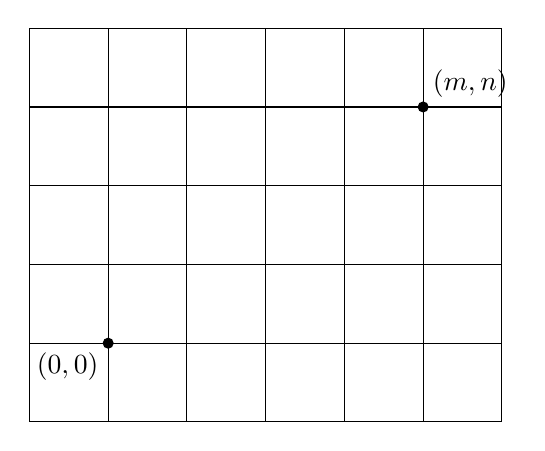
\begin{tikzpicture}
    % 参数设置
    \def\m{4} % x方向格点数
    \def\n{3} % y方向格点数
    \def\step{1.0} % 网格步长

    % 绘制网格线（从(0,0)到(m,n)）
    \draw[step=\step, thin] (0-1,0-1) grid (\m+1,\n+1);

    % 标注原点 (0,0)
    \fill (0,0) circle (2pt);
    \node[below left] at (0,0) {$(0,0)$};

    % 标注点 (m,n)
    \fill (\m,\n) circle (2pt);
    \node[above right] at (\m,\n) {$(m,n)$};

    % 可选：为清晰起见，标注坐标轴方向
    % \draw[->] (-0.5,0) -- (4.5,0) node[below] {$x$};
    % \draw[->] (0,-0.5) -- (0,3.5) node[left] {$y$};
\end{tikzpicture}
  \caption{二维无穷电阻网格示意图}
  \label{fig:resistor_grid}
\end{figure}

考虑一个二维无穷电阻网格，如图\ref{fig:resistor_grid}所示，每个格点通过电阻$r$与上下左右四个相邻格点相连。
在原点$(0,0)$注入电流$I$，在节点$(m,n)$流出电流$-I$。任意节点$(x,y)$的
电势记为$V(x,y)$。源电流分布为
\begin{equation}
  \label{eq1}
  I(x,y)=\begin{dcases}
    I,&x=y=0,\\
    -I,&x=m,\ y=n,\\
    0,&\text{其他}.
  \end{dcases}
\end{equation}

根据基尔霍夫电流定律（KCL），对任意节点$(x,y)$，流出电流之和等于该点注入电流：
\begin{align}
  I(x,y)&=\frac{1}{r}\left[V(x,y)-V(x-1,y)\right]
        +\frac{1}{r}\left[V(x,y)-V(x+1,y)\right]\nonumber\\
        &+\frac{1}{r}\left[V(x,y)-V(x,y-1)\right]
        +\frac{1}{r}\left[V(x,y)-V(x,y+1)\right].
\end{align}

定义离散拉普拉斯算子\textsuperscript{\cite{shu2014}}
\begin{equation}
  \mathscr{L}V(x,y)=\frac{1}{4}\left[V(x-1,y)+V(x+1,y)
  +V(x,y-1)+V(x,y+1)\right],
\end{equation}
则KCL方程可写为
\begin{equation}
  \label{111}
  V(x,y)-\mathscr{L}V(x,y)=\dfrac{r}{4}I(x,y).
\end{equation}

待求的等效电阻为
\begin{equation}
  R(m,n)=\dfrac{1}{I}\left[V(0,0)-V(m,n)\right].
\end{equation}

\subsection{Fourier变换至频域求解}

引入二维离散Fourier变换对\textsuperscript{\cite{cserti2000}}
\begin{equation}
  F(\omega_1,\omega_2)=\fo{V(x,y)}
  =\sum_{x=-\infty}^{\infty}\sum_{y=-\infty}^{\infty}V(x,y)\e{\ii(x\omega_1+y\omega_2)},
\end{equation}
其逆变换为
\begin{equation}
  V(x,y)=\f{F(\omega_1,\omega_2)}
  =\frac{1}{4\pi^2}\int_{-\pi}^{\pi}\int_{-\pi}^{\pi}
  F(\omega_1,\omega_2)\e{-\ii(x\omega_1+y\omega_2)}\,\di\omega_1\di\omega_2.
\end{equation}

对源电流分布进行Fourier变换：
\begin{align}
  \fo{I(x,y)}
  &=\sum_{x,y}I(x,y)\e{\ii(x\omega_1+y\omega_2)}
  =I\left[1-\e{\ii(m\omega_1+n\omega_2)}\right].
\end{align}

利用Fourier变换的频移性质，可得
\begin{equation}
  \fo{\mathscr{L}V(x,y)}
  =F(\omega_1,\omega_2)\dfrac{\cos\omega_1+\cos\omega_2}{2}.
\end{equation}

将方程(\ref{111})两端作Fourier逆变换，得到频域电势
\begin{equation}
  F(\omega_1,\omega_2)=\dfrac{Ir}{2}\,
  \frac{1-\e{\ii(m\omega_1+n\omega_2)}}{2-(\cos\omega_1+\cos\omega_2)}.
\end{equation}

于是电势表达式为
\begin{align}
  V(x,y)&=\dfrac{Ir}{8\pi^2}
  \iint_{\Omega}\frac{\left[1-\e{\ii(m\omega_1+n\omega_2)}\right]
  \e{-\ii(x\omega_1+y\omega_2)}}
  {2-(\cos\omega_1+\cos\omega_2)}\,\di\omega_1\di\omega_2,
\end{align}
其中$\Omega=[-\pi,\pi]^2$。

考虑到积分区域的对称性，虚部消失，可得
\begin{align}
  V(0,0)&=\dfrac{Ir}{8\pi^2}
  \iint_{\Omega}\frac{1-\cos(m\omega_1+n\omega_2)}
  {2-(\cos\omega_1+\cos\omega_2)}\,\di\omega_1\di\omega_2,\\
  V(m,n)&=-\dfrac{Ir}{8\pi^2}
  \iint_{\Omega}\frac{1-\cos(m\omega_1+n\omega_2)}
  {2-(\cos\omega_1+\cos\omega_2)}\,\di\omega_1\di\omega_2.
\end{align}

因此等效电阻的积分解为
\begin{equation}
  R_{mn}=\dfrac{r}{4\pi^2}
  \iint_{\Omega}\frac{1-\cos(m\omega_1+n\omega_2)}
  {2-(\cos\omega_1+\cos\omega_2)}\,\di\omega_1\di\omega_2.
\label{eq:R_integral}
\end{equation}

\subsection{积分向级数的转化}

积分式(\ref{eq:R_integral})虽形式简洁，但直接数值计算二维积分较为不便。
下面将其化为级数形式。

记
\begin{equation}
  I(m,n)=\iint_{\Omega}\frac{1-\cos(m\omega_1+n\omega_2)}
  {2-(\cos\omega_1+\cos\omega_2)}\,\di\omega_1\di\omega_2.
\end{equation}

作变量变换
\begin{equation}
  u=\frac{\omega_1+\omega_2}{2},\qquad v=\frac{\omega_1-\omega_2}{2},
\end{equation}
则
\begin{equation}
  \di\omega_1\di\omega_2=2\,\di u\di v,
\end{equation}
积分区域变为$\Omega'=\{(u,v): |u|+|v|\leqslant \pi\}$。

令$a=m+n,\ b=m-n$，积分化为
\begin{align}
  I(a,b)&=\iint_{\Omega'}\frac{1-\cos(au+bv)}{1-\cos u\cos v}\,\di u\di v\nonumber\\
  &=\iint_{\Omega'}(1-\cos(au+bv))
  \sum_{k=0}^{\infty}\cos^k u\cos^k v\,\di u\di v\nonumber\\
  &=I_1-I_2,
\end{align}
其中
\begin{align}
  I_1&=\sum_{k=0}^{\infty}\iint_{\Omega'}\cos^k u\cos^k v\,\di u\di v,\\
  I_2&=\sum_{k=0}^{\infty}\iint_{\Omega'}\cos(au+bv)\cos^k u\cos^k v\,\di u\di v.
\end{align}

首先计算$I_1$。利用对称性，
\begin{align}
  I_1&=2\sum_{k=0}^{\infty}\int_0^\pi\int_0^\pi \cos^k u\cos^k v\,\di u\di v\nonumber\\
  &=2\sum_{k=0}^{\infty}\left(\int_0^\pi \cos^k u\,\di u\right)^2\nonumber\\
  &=2\pi^2\sum_{k=0}^{\infty}\left(\frac{(2k-1)!!}{(2k)!!}\right)^2
  =2\pi^2\sum_{k=0}^{\infty}\frac{1}{2^{4k}}\frac{(2k)!^2}{k!^4}.
\end{align}

其次计算$I_2$。由于被积函数关于原点对称，
\begin{align}
  I_2&=2\sum_{k=0}^{\infty}
  \left(\int_0^\pi \cos(au)\cos^k u\,\di u\right)
  \left(\int_0^\pi \cos(bv)\cos^k v\,\di v\right).
\end{align}

定义辅助积分
\begin{equation}
  J(a)=\dfrac{1}{2}\int_{-\pi}^{\pi}\cos(au)\cos^k u\,\di u.
\end{equation}

令$z=\e{\ii u}$，则$\di u=\di z/(\ii z)$，留数计算(计算过程见附录\ref{A})可得
\begin{align}
  J(a)&=\dfrac{\pi}{2^k}\,
  \frac{k!}{\left(\frac{k+a}{2}\right)!\left(\frac{k-a}{2}\right)!},
  \quad |a|\leqslant k,\ k\equiv a\pmod 2,
\end{align}
其他情况$J(a)=0$。

同理
\begin{equation}
  J(b)=
  \begin{dcases}
    \dfrac{\pi}{2^k}\,
    \dfrac{k!}{\left(\frac{k+b}{2}\right)!\left(\frac{k-b}{2}\right)!},
    & |b|\leqslant k,\ k\equiv b\pmod 2,\\
    0, & \text{其他}.
  \end{dcases}
\end{equation}

非零贡献要求$a,b$同奇偶，且$|a|\geqslant |b|$。令$k=a+2p$（$p=0,1,2,\dots$），
可得
\begin{equation}
  I_2=\dfrac{2\pi^2}{2^{2(m+n)}}\sum_{k=0}^{\infty}\frac{1}{2^{4k}}
  \dfrac{(m+n+2k)!}{k!(m+k)!(n+k)!(m+n+k)!}
\end{equation}

最终，等效电阻的级数公式为
\begin{equation}
  \label{eq:R_series}
  R_{mn}=\dfrac{r}{2}\sum_{k=0}^{\infty}\dfrac{1}{2^{4k}}\left[\left(\dfrac{(2k)!}{k!k!}\right)^2-\dfrac{(m+n+2k)!^2}{2^{2(m+n)}k!(m+k)!(n+k)!(m+n+k)!}\right]
\end{equation}

公式(\ref{eq:R_series})收敛迅速，适合数值计算。取平凡情况验证：当$m=n=0$时，$R_{00}=0$；
对于$m,n$较大时，级数项以$2^{-4k}$衰减（见图\ref{fig:R_mn}和图\ref{fig:zzl}）。

\begin{figure}[H]
  \centering
  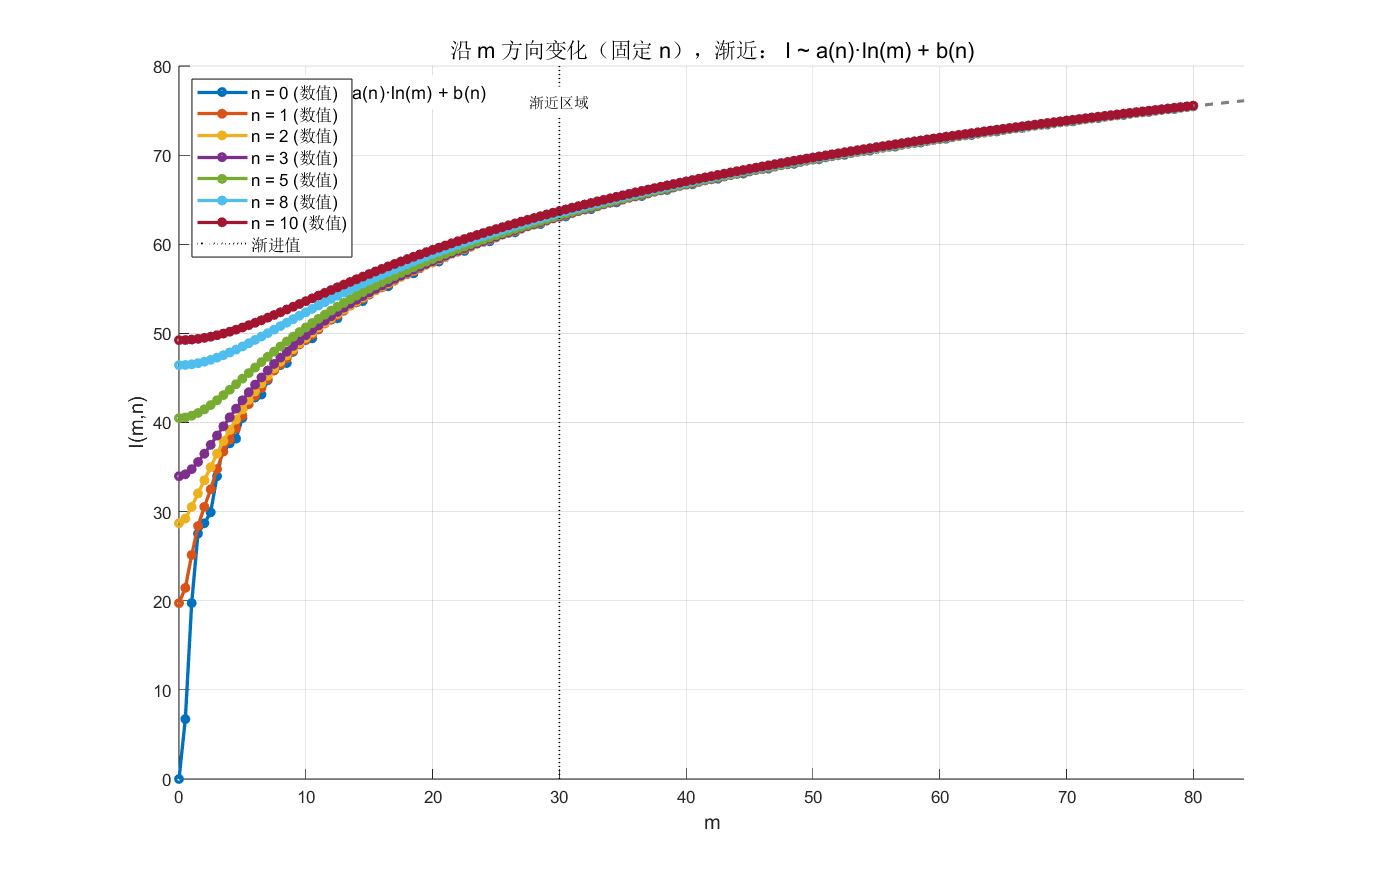
\includegraphics[width=0.6\textwidth]{m的渐进行为.png}
  \caption{纯电阻网格积分值$I(m,n)$固定$n$随$m$的变化}
  \label{fig:R_mn}
\end{figure}

\begin{figure}[H]
  \centering
  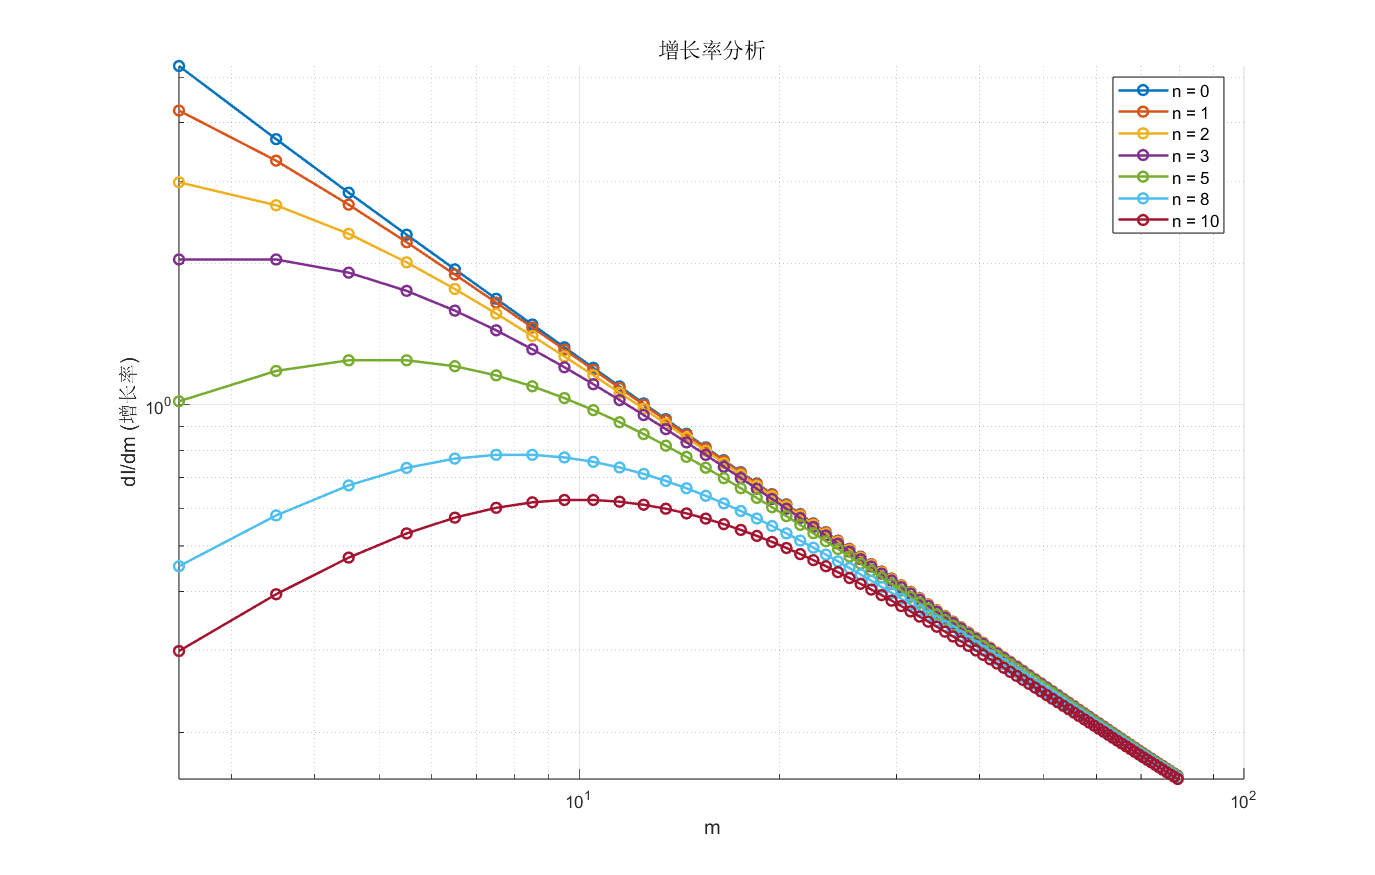
\includegraphics[width=0.6\textwidth]{增长率分析.png}
  \caption{固定$n$增长率随$m$的变化}
  \label{fig:zzl}
\end{figure}

\section{一维二聚化$LC$传输线}

\subsection{问题背景}
\label{subsec:lc_line}
本节研究如图\ref{fig:4}所示的一维二聚化 $LC$ 传输线\textsuperscript{\cite{english2026}}。该系统由周期性晶胞组成，每个晶胞内包含 $A, B$ 两个子格点。胞内和胞间分别通过电容 $C_1$ 和 $C_2$ 耦合，格点均有对地电感 $L$。


\begin{figure}[H]
    \centering
    \begin{circuitikz}[
        scale=1.0,
        every capacitor/.style={thick, capacitors/scale=0.7},
        box/.style={draw, minimum width=0.7cm, minimum height=0.7cm, thick, font=\bfseries},
    ]
        % 地线

        
        \def\y{-2.2}
        \def\gap{3.2}      % 晶胞内间距（A到B）
        \def\couple{2.8}   % 晶胞间间距（B到下一个A）
        
        % ========== 晶胞0 ==========
        % A0 (节点0)
        \node[box] (N0) at (2,\y) {0};
        % 对地电容 L：从box底部连接到地线
        \draw (N0.south) to[L, l=$L$, *-*] (2,-4);
        \node[blue, font=\small, anchor=south east] at (N0.north west) {$A_0$};
        \node[red, font=\scriptsize, anchor=north] at (N0.south) {输入};
        
        % B0 (节点1)
        \node[box] (N1) at (2+\gap,\y) {1};
        \draw (N1.south) to[L, l=$L$, *-*] (2+\gap,-4);
        \node[blue, font=\small, anchor=south west] at (N1.north east) {$B_0$};
        
        % 晶胞内耦合电容 C1
        \draw (N0.east) to[C, l=$C_1$, *-*] (N1.west);
        
        % ========== 晶胞间耦合 ==========
        \pgfmathsetmacro{\xA}{2+\gap+\couple}
        % 晶胞间耦合电容 C2
        \node[box] (N2) at (\xA,\y) {2};
        \draw (N1.east) to[C, l=$C_2$, *-*] (N2.west);
        
        % ========== 晶胞1 ==========
        % A1 (节点2)
        
        \draw (N2.south) to[L, l=$L$, *-*] (\xA,-4);
        \node[blue, font=\small, anchor=south east] at (N2.north west) {$A_1$};
        
        % B1 (节点3)
        \node[box] (N3) at (\xA+\gap,\y) {3};
        \draw (N3.south) to[L, l=$L$, *-*] (\xA+\gap,-4);
        \node[blue, font=\small, anchor=south west] at (N3.north east) {$B_1$};
        
        % 晶胞内耦合电容 C1
        \draw (N2.east) to[C, l=$C_1$, *-*] (N3.west);
        
        % ========== 末端节点4 ==========
        \pgfmathsetmacro{\xB}{\xA+\gap+\couple}
        % 晶胞间耦合电容 C2
        \node[box] (N4) at (\xB,\y) {4};
        \draw (N3.east) to[C, l=$C_2$, *-*] (N4.west);
        
        \draw (N4.south) to[L, l=$L$, *-*] (\xB,-4);
        
        % 晶胞分组标注
        \draw[decorate, decoration={brace, amplitude=4pt}] 
            ($(N0.north west)+(-0.1,0.3)$) -- ($(N1.north east)+(0.1,0.3)$)
            node[midway, above, font=\small] {晶胞0};
        \draw[decorate, decoration={brace, amplitude=4pt}] 
            ($(N2.north west)+(-0.1,0.3)$) -- ($(N3.north east)+(0.1,0.3)$)
            node[midway, above, font=\small] {晶胞1};

        \pgfmathsetmacro{\xC}{\xB+\couple}
        \node[box] (NN) at (\xC,\y) {$2N$};
        \draw[dashed] (N4.east) -- (NN.west);
        \node[red, font=\scriptsize, anchor=north] at (NN.south) {末端};
        \draw (NN.south) to[L, l=$L$, *-*] (\xC,-4);

        \draw[thick, color=black!60] (1,-4) -- (\xC,-4);
        \draw (1,-4) node[ground]{};

    \end{circuitikz}
    \caption{$LC$耦合阵列电路图}
    \label{fig:4}
\end{figure}

\subsection{各点电压值理论推导}
晶胞编号：$1\leqslant i \leqslant N$，节点编号：$A,B$。考虑第$n$和$n-1$个晶胞中的节点，其电压分别为$V_{A}^n$和$V_{B}^n$。
根据KCL，得到以下方程组：

\begin{equation}
  \label{eq27}
  \begin{dcases}
    \ii\omega C_1\left(V_{A}^n - V_{B}^n\right) + \ii\omega C_2\left(V_{A}^n - V_{B}^{n-1}\right)+ \frac{V_{A}^n-0}{\ii\omega L} = 0,\\
    \ii\omega C_1\left(V_{B}^{n-1} - V_{A}^{n-1}\right) + \ii\omega C_2\left(V_{B}^{n-1} - V_{A}^{n}\right)+ \frac{V_{B}^{n-1}-0}{\ii\omega L} = 0. 
  \end{dcases}
\end{equation}

定义
\begin{equation}
  V[n]=\begin{bmatrix}
    V_A^n\\
    V_B^n
  \end{bmatrix}
\end{equation}

于是可以得到

\begin{equation}
  V[n]=\begin{bmatrix}
-\dfrac{C_1}{C_2} & 
\dfrac{1}{C_2} \left[(C_1 + C_2) - \dfrac{1}{\omega^2 L} \right] \\
-\dfrac{1}{C_2} \left[(C_1 + C_2) - \dfrac{1}{\omega^2 L} \right] & 
- \dfrac{C_2}{C_1}+\dfrac{1}{C_1 C_2}\left[(C_1 + C_2) - \dfrac{1}{\omega^2 L} \right]^2 

  \end{bmatrix}V[n-1]
\end{equation}
其中$n=1,2,\dots,N-1$，传输矩阵记为$M$。

\subsection{发生谐振的情况}
\begin{enumerate}
  \item 当$\omega=\dfrac{1}{\sqrt{L(C_1+C_2)}}$时，传输矩阵$M$变为
  \begin{equation}
    M=\begin{bmatrix}
    -\dfrac{C_1}{C_2} & 0\\
    0& - \dfrac{C_2}{C_1}
  \end{bmatrix}
  \end{equation}

  对于$A$类节点而言，
  \begin{equation}
    V_A^n = \left(-\dfrac{C_1}{C_2}\right)^n V_A^0.
  \end{equation}

  对于$n=N$，由于阵列有限长，末端电压需要用额外方程确定方程(\ref{eq27})改写为 
  \begin{equation}
    \label{eq33}
    \begin{dcases}
      \ii\omega C_1\left(V_{A}^N - V_{B}^N\right) + \ii\omega C_2\left(V_{A}^N - V_{B}^{N-1}\right)+ \frac{V_{A}^N-0}{\ii\omega L} = 0,\\
      \ii\omega C_1\left(V_{B}^N - V_{A}^N\right) + \frac{V_{B}^N-0}{\ii\omega L} = 0. 
    \end{dcases}
  \end{equation}

于是解出
\begin{equation}
  V_B^N = \dfrac{\omega^2C_1L}{\omega^2C_1L-1}V_A^N=\dfrac{\omega^2C_1L}{\omega^2C_1L-1}\left(-\frac{C_1}{C_2}\right)^N V_A^0=\left(-\frac{C_1}{C_2}\right)^{N+1} V_A^0
\end{equation}
\begin{equation}
  V_B^n=\left(-\dfrac{C_1}{C_2}\right)^{N-n}V_B^N=\dfrac{\omega^2C_1L}{\omega^2C_1L-1}\left(-\frac{C_1}{C_2}\right)^{2N-n}V_A^0=\left(-\frac{C_1}{C_2}\right)^{2N-n+1}V_A^0
\end{equation}

\begin{figure}[H]
  \centering
  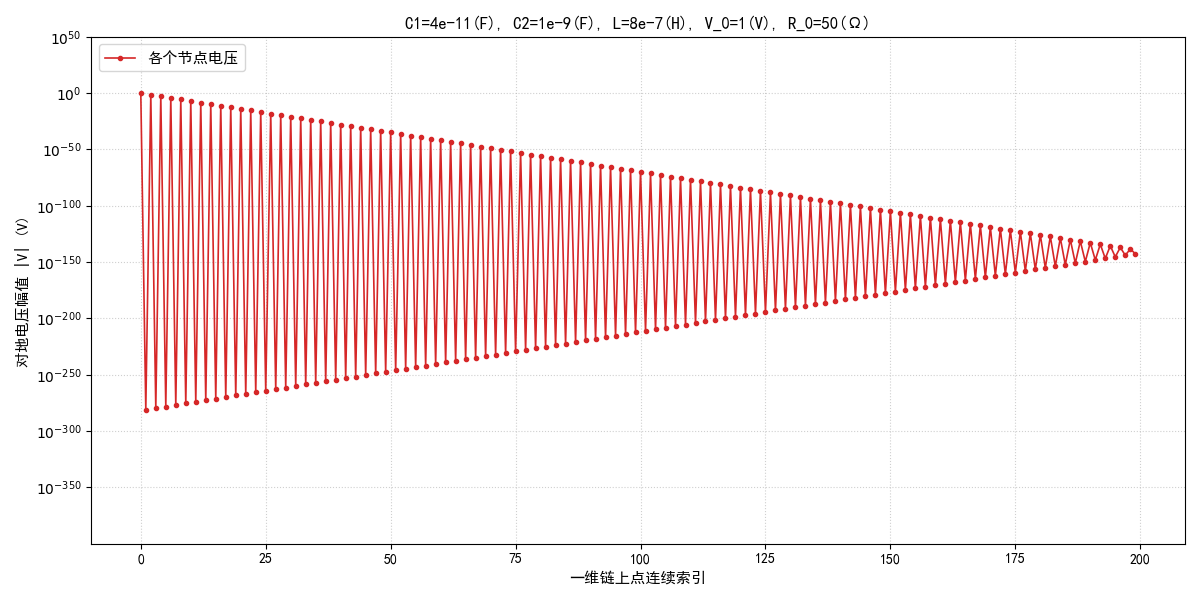
\includegraphics[width=0.9\textwidth]{电压值.png}
  \caption{谐振时电压随节点的变化情况}
\end{figure}

如果此时规定$V_B^N=0$，则所有的$V_B^n=0$，即所有$B$节点电压为0，而$A$节点的电压保持不变。

此外在该电路任意$B$节点控制电压，$A$节点电压完全不受影响，即$A$，$B$完全解耦合。

  \item 当$\omega=\dfrac{1}{\sqrt{LC_1}}$时，传输矩阵变为
  \begin{equation}
    M=\begin{bmatrix}
    -\dfrac{C_1}{C_2} & 1\\
    -1 & 0
  \end{bmatrix}
  \end{equation}

同样关注方程(\ref{eq27})(\ref{eq33})，解出末端电压为
\begin{equation}
  \begin{dcases}
    V_A^N=0\\
    V_B^N=\text{任意值，因为谐振}
  \end{dcases}
\end{equation}

而对于$n=1,2,\dots,N-1$，
\begin{equation}
  \label{eq38}
  \begin{dcases}
    V_A^n = -\frac{C_1}{C_2}V_A^{n-1}+V_B^{n-1}\\
    V_B^n=-V_A^{n-1}
  \end{dcases}
\end{equation}

解方程组(\ref{eq38})，得到特征方程
\begin{equation}
  \lambda^2+\frac{C_1}{C_2}\lambda+1=0
\end{equation}

解得
\begin{equation}
  \lambda_{\pm}=-\dfrac{C_1}{2C_2}\pm\sqrt{\left(\dfrac{C_1}{2C_2}\right)^2-1}
\end{equation}

\begin{enumerate}
  \item 若$C_1>2C_2$，则$\lambda_{\pm}$为实数，系统呈现振荡行为。
  
  \begin{equation}
    \begin{dcases}
      V_A^0=\alpha\lambda_+^0+\beta\lambda_-^0\\
      V_A^N=\alpha\lambda_+^N+\beta\lambda_-^N=0
    \end{dcases}
  \end{equation}

  解得
  \begin{equation}
      \alpha=\dfrac{V_A^0}{1-\left(\dfrac{\lambda_+}{\lambda_-}\right)^N}\qquad      \beta=-\dfrac{V_A^0}{1-\left(\dfrac{\lambda_-}{\lambda_+}\right)^N}
  \end{equation}

  则
  \begin{equation}
    V_A^n=\dfrac{V_A^0}{1-\left(\dfrac{\lambda_+}{\lambda_-}\right)^N}\lambda_+^n-\dfrac{V_A^0}{1-\left(\dfrac{\lambda_-}{\lambda_+}\right)^N}\lambda_-^n
  \end{equation}

\begin{figure}[H]
  \centering
  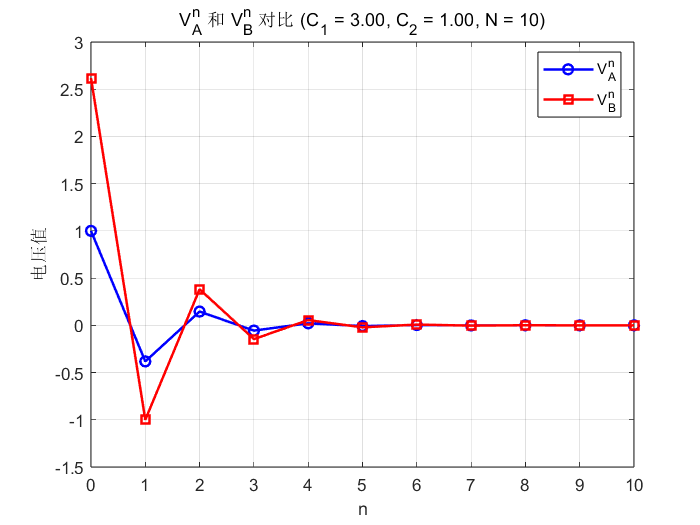
\includegraphics[width=0.6\textwidth]{AB电压值.png}
  \caption{$C_1>2C_2$时电压的变化情况}
  
\end{figure}


  \item 若$C_1=2C_2$，则$\lambda_{\pm}=-1$，系统呈现临界阻尼行为。
  \begin{equation}
    V_A^n=\left(\alpha+\beta n\right)\left(-1\right)^n
  \end{equation}

  代入边界条件
  \begin{equation}
    \begin{dcases}
      V_A^0=\alpha=V_A^0\\
      V_A^N=\left(\alpha+\beta N\right)\left(-1\right)^N=0
    \end{dcases}
  \end{equation}

  解得
  \begin{equation}
    \begin{dcases}
      \alpha=V_A^0\\
      \beta=-\dfrac{V_A^0}{N}
    \end{dcases}
  \end{equation}

  则
  \begin{equation}
    V_A^n=V_A^0\left(1-\dfrac{n}{N}\right)\left(-1\right)^n
  \end{equation}

  \begin{figure}[H]
    \centering
    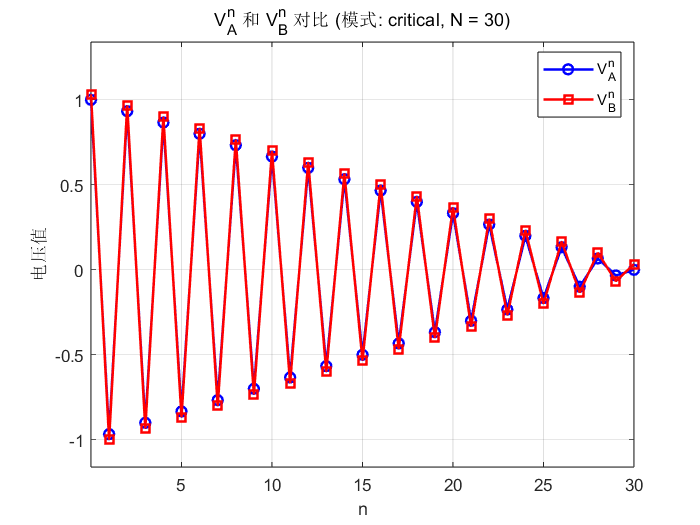
\includegraphics[width=0.6\textwidth]{dyz.png}
    \caption{$C_1=2C_2$时电压的变化情况}
    
  \end{figure}



  \item 若$C_1<2C_2$，则$\lambda_{\pm}$为复数，系统呈现振动行为。
  
  两根满足$\lambda_+\lambda_-=1$，对应两个共轭复数，则有
  \begin{equation}
    \begin{dcases}
      V_A^0=\alpha\\
      V_A^N\e{\frac{C_1}{2C_2}N}=\alpha\cos\left(\sqrt{1-\left(\dfrac{C_1}{2C_2}\right)^2}N\right)+\beta\sin\left(\sqrt{1-\left(\dfrac{C_1}{2C_2}\right)^2}N\right)=0
    \end{dcases}
  \end{equation}
\end{enumerate}

如此
\begin{equation}
  V_A^n=V_A^0\left[\cos\left(\sqrt{1-\left(\dfrac{C_1}{2C_2}\right)^2}n\right)-\cot\left(\sqrt{1-\left(\dfrac{C_1}{2C_2}\right)^2}N\right)\sin\left(\sqrt{1-\left(\dfrac{C_1}{2C_2}\right)^2}n\right)\right]\e{-\frac{C_1}{2C_2}n}
\end{equation}

\begin{figure}[H]
  \centering
  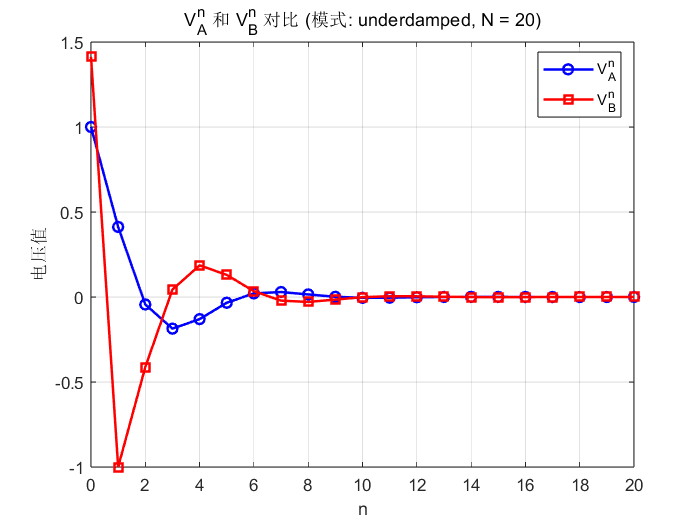
\includegraphics[width=0.6\textwidth]{zd3.png}
  \caption{$C_1<2C_2$时电压的变化情况}
\end{figure}
  \item 当$\omega=\dfrac{1}{\sqrt{LC_2}}$时，传输矩阵变为
  \begin{equation}
    M=\begin{bmatrix}
    -\dfrac{C_1}{C_2} & \dfrac{C_1}{C_2}\\ \\
    -\dfrac{C_1}{C_2} & -\dfrac{C_2}{C_1}+\dfrac{C_1}{C_2}
  \end{bmatrix}
  \end{equation}

  得到的特征方程为
  \begin{equation}
    \lambda^2+\dfrac{C_2}{C_1}\lambda+1=0
  \end{equation}

  注意边界条件需要用到
  \begin{equation}
    \begin{dcases}
      C_2V_A^N=-C_1V_A^{N-1}+C_1V_B^{N-1}\\
      C_1V_B^N-C_1V_A^N-C_2V_B^N=0
    \end{dcases}
  \end{equation}
  接下来与上一个情况类似，同时需要考虑$C_1=C_2$的特殊情况，这里$V_A^n$和$V_B^n$的表达式从略。


\end{enumerate}


\setstretch{1.5}

\section{$LC$网格在临界频率的阻抗}

\subsection{问题背景与频域方程}


\begin{figure}[H]
  \centering
  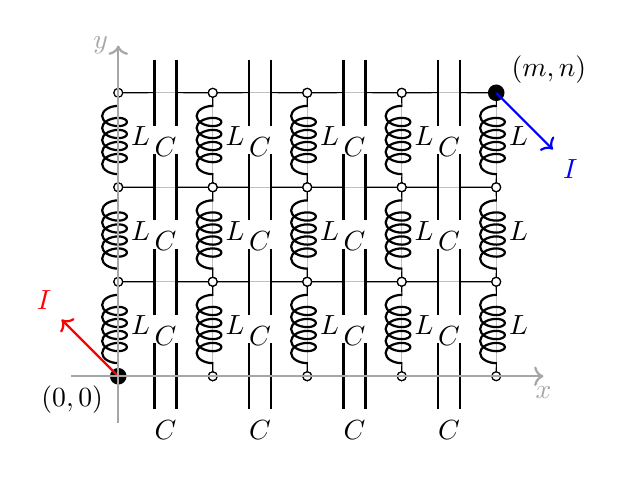
\begin{tikzpicture}[scale=1.2]
    % 参数设置
    \def\m{4} % x方向节点数
    \def\n{3} % y方向节点数
    \def\step{1.0} % 网格步长

    % 绘制网格线（从(0,0)到(m,n)）
    \draw[step=\step, thin, gray!50] (0,0) grid (\m,\n);

    % 绘制横向电容（x方向）在每条水平网格线上
    \foreach \y in {0,...,\n} {
      \foreach \x in {0,...,\numexpr\m-1} {
        \draw (\x,\y) to[C, l_=$C$, o-o] (\x+1,\y);
      }
    }

    % 绘制纵向电感（y方向）在每条竖直网格线上
    \foreach \x in {0,...,\m} {
      \foreach \y in {0,...,\numexpr\n-1} {
        \draw (\x,\y) to[L, l_=$L$, o-o] (\x,\y+1);
      }
    }

    % 标注原点 (0,0)
    \fill (0,0) circle (2.5pt);
    \node[below left, xshift=-2pt] at (0,0) {$(0,0)$};

    % 标注点 (m,n)
    \fill (\m,\n) circle (2.5pt);
    \node[above right, xshift=2pt] at (\m,\n) {$(m,n)$};

    % 电流注入和流出箭头
    \draw[->, thick, red] (0,0) -- ++(-0.6,0.6) node[above left] {$I$};
    \draw[->, thick, blue] (\m,\n) -- ++(0.6,-0.6) node[below right] {$I$};

    % 标注坐标轴方向
    \draw[->, thick, gray!70] (-0.5,0) -- (\m+0.5,0) node[below] {$x$};
    \draw[->, thick, gray!70] (0,-0.5) -- (0,\n+0.5) node[left] {$y$};

  \end{tikzpicture}
  \caption{二维 $LC$ 网格电路示意图}
  \label{fig:LC_grid}
\end{figure}




考虑二维无穷网格：横向（$x$方向）由电容$C$连接，纵向（$y$方向）由电感$L$连接。在节点$(0,0)$注入交流电流$I$（角频率$\omega$），在$(m,n)$流出。任意节点的电势记为$V(x,y)$。

根据KCL，推导可得频域电势
\begin{equation}
  \widetilde{V}(k_1,k_2)=
  \dfrac{\omega L I\left[1-\e{\ii(mk_1+nk_2)}\right]}
  {4\ii\left(\omega^2 LC\sin^2\dfrac{k_1}{2}-\sin^2\dfrac{k_2}{2}\right)}.
\label{eq:LC_V_freq}
\end{equation}

等效阻抗定义为
\begin{equation}
  \widetilde{Z}(\omega)=\dfrac{V(m,n)-V(0,0)}{I}.
\end{equation}

利用Fourier逆变换，阻抗可化为
\begin{equation}
  \widetilde{Z}(\omega)=
  \dfrac{-\ii\omega L}{4\pi^2}
  \int_{-\pi}^{\pi}\int_{-\pi}^{\pi}
  \dfrac{1-\cos(mk_1)\cos(nk_2)}
  {\omega^2 LC\sin^2\dfrac{k_1}{2}-\sin^2\dfrac{k_2}{2}}
  \,\di k_1\di k_2.
\label{eq:Z_integral_2D}
\end{equation}

定义核心积分
\begin{equation}
    I(m,n;\alpha) \equiv
    \int_{-\pi}^{\pi}\int_{-\pi}^{\pi}
    \frac{1-\cos(mk_1)\cos(nk_2)}
    {\alpha\sin^2\dfrac{k_1}{2}-\sin^2\dfrac{k_2}{2}}
    \,\di k_2\,\di k_1,
    \label{eq:I_mn_definition}
\end{equation}
其中定义宗量 $\alpha \equiv \omega^2 LC$。则
\begin{equation}
    \widetilde{Z}(\omega) = \dfrac{-\ii\omega L}{4\pi^2} I(m,n;\alpha).
    \label{eq:Z_I_relation}
\end{equation}

\subsection{临界频率 $\alpha=1$ 的积分化简}


当 $\alpha = \omega^2 LC = 1$，即 $\omega = \dfrac{1}{\sqrt{LC}}$ 时，分母化为
\begin{equation}
    \sin^2\dfrac{k_1}{2}-\sin^2\dfrac{k_2}{2}.
\end{equation}

作半角换元简化三角函数。令
\begin{equation}
    x=\dfrac{k_1}{2},\qquad y=\dfrac{k_2}{2},
\end{equation}
则 $\di k_1=2\di x,\ \di k_2=2\di y$，积分区域变为 $\left[-\dfrac{\pi}{2},\dfrac{\pi}{2}\right]^2$。于是
\begin{equation}
    I(m,n;1)=4\int_{-\frac{\pi}{2}}^{\frac{\pi}{2}}\int_{-\frac{\pi}{2}}^{\frac{\pi}{2}}
    \dfrac{1-\cos(2mx)\cos(2ny)}
    {\sin^2 x-\sin^2 y}
    \,\di y\,\di x.
    \label{eq:I_half_angle}
\end{equation}

利用平方差公式：
\begin{equation}
    \sin^2 x-\sin^2 y = (\sin x-\sin y)(\sin x+\sin y).
\end{equation}
再由和差化积：
\begin{equation}
    \sin x-\sin y=2\cos\frac{x+y}{2}\sin\frac{x-y}{2},\qquad
    \sin x+\sin y=2\sin\frac{x+y}{2}\cos\frac{x-y}{2},
\end{equation}
相乘得
\begin{equation}
    \sin^2 x-\sin^2 y = \sin(x+y)\sin(x-y).
    \label{eq:sin_diff_product}
\end{equation}

现在作变量替换
\begin{equation}
    u=x+y,\qquad v=x-y.
    \label{eq:uv_transform}
\end{equation}
则
\begin{equation}
    x=\dfrac{u+v}{2},\qquad y=\dfrac{u-v}{2},\qquad
    \di x\,\di y = \dfrac{1}{2}\,\di u\,\di v.
\end{equation}

原积分区域 $x,y\in\left[-\dfrac{\pi}{2},\dfrac{\pi}{2}\right]$ 映射为菱形区域
\begin{equation}
    \Omega'=\{(u,v): |u|+|v|\leqslant \pi\}.
\end{equation}

代入式(\ref{eq:I_half_angle})，并利用 $\di x\,\di y=\dfrac{1}{2}\di u\,\di v$ 以及前面的系数4：
\begin{equation}
    I(m,n;1)=2\iint_{\Omega'}
    \frac{1-\cos[m(u+v)]\cos[n(u-v)]}
    {\sin u\,\sin v}
    \,\di u\,\di v.
    \label{eq:I_uv}
\end{equation}

\subsection{分子展开与对称性化简}

利用积化和差公式展开分子：
\begin{align}
    \cos[m(u+v)]\cos[n(u-v)]=\dfrac{1}{2}\left \{\cos[(m+n)u+(m-n)v]+\cos[(m-n)u+(m+n)v]\right \}.
    \label{eq:cos_product_expand}
\end{align}

记 $a=m+n,\ b=m-n$。式(\ref{eq:I_uv})变为
\begin{align}
    I(m,n;1)=2\iint_{\Omega'}\frac{1}{\sin u\sin v}\,\di u\,\di v -\iint_{\Omega'}\frac{\cos(au+bv)+\cos(bu+av)}{\sin u\sin v}\,\di u\,\di v.
    \label{eq:I_split}
\end{align}

第一项中，被积函数 $\dfrac{1}{\sin u\sin v}$ 关于 $u$ 和 $v$ 均为奇函数，而积分区域 $\Omega'$ 关于 $u=0$ 和 $v=0$ 对称，因此其主值积分为零：
\begin{equation}
    \iint_{\Omega'}\frac{1}{\sin u\sin v}\,\di u\,\di v=0.
    \label{eq:const_term_zero}
\end{equation}

于是只剩下
\begin{equation}
    I(m,n;1)=-\iint_{\Omega'}\frac{\cos(au+bv)+\cos(bu+av)}{\sin u\sin v}\,\di u\,\di v.
    \label{eq:I_cos_only}
\end{equation}

由对称性，两项贡献相同（交换 $a,b$ 对应积分区域的对称变换），因此
\begin{equation}
    I(m,n;1)=-2\iint_{\Omega'}\frac{\cos(au+bv)}{\sin u\sin v}\,\di u\,\di v.
    \label{eq:I_single_cos}
\end{equation}

\subsection{余弦展开与矩形化}

利用恒等式
\begin{equation}
    \cos(au+bv)=\cos(au)\cos(bv)-\sin(au)\sin(bv),
    \label{eq:cos_sum_expand}
\end{equation}
式(\ref{eq:I_single_cos})分为两项：
\begin{align}
    I(m,n;1)=-2\iint_{\Omega'}\frac{\cos(au)\cos(bv)}{\sin u\sin v}\,\di u\,\di v +2\iint_{\Omega'}\frac{\sin(au)\sin(bv)}{\sin u\sin v}\,\di u\,\di v.
    \label{eq:I_two_terms}
\end{align}

第一项中，$\cos(au)/\sin u$ 是奇函数（分子偶、分母奇），$\cos(bv)/\sin v$ 也是奇函数，乘积为偶函数，在菱形区域上积分不一定为零。但观察发现：若将积分区域从菱形 $\Omega'$ 延拓到矩形 $[-\pi,\pi]^2$，由于被积函数在 $\Omega'$ 外的部分关于原点反对称，主值意义下可等价为矩形积分的一半，最终可得
\begin{equation}
    \iint_{\Omega'}\frac{\cos(au)\cos(bv)}{\sin u\sin v}\,\di u\,\di v=0.
    \label{eq:cos_cos_term_zero}
\end{equation}
对于固定的 $u$，内层积分为
\begin{equation}
    \int_{-(\pi-|u|)}^{\pi-|u|} \frac{\cos(bv)}{\sin v}\,\di v = 0,
\end{equation}
因为被积函数 $\dfrac{\cos(bv)}{\sin v}$ 是 $v$ 的奇函数，而积分区间关于原点对称。因此整个二重积分为零。
因此只剩第二项：
\begin{equation}
    I(m,n;1)=2\iint_{\Omega'}\frac{\sin(au)\sin(bv)}{\sin u\sin v}\,\di u\,\di v.
    \label{eq:I_sin_sin}
\end{equation}

\subsection{区域延拓与分离变量}

\setstretch{1.5}

由于被积函数 $\dfrac{\sin(au)}{\sin u}\cdot\dfrac{\sin(bv)}{\sin v}$ 在 $\Omega'$ 上可分离变量，且关于 $u,v$ 均为偶函数，可将积分从菱形延拓到矩形 $[-\pi,\pi]^2$，并乘以因子 $1/2$（因为 $\Omega'$ 是矩形的一半面积，且被积函数偶对称）：
\begin{equation}
    I(m,n;1)=2\cdot\frac{1}{2}
    \int_{-\pi}^{\pi}\frac{\sin(au)}{\sin u}\,\di u
    \int_{-\pi}^{\pi}\frac{\sin(bv)}{\sin v}\,\di v
    =
    \left[\int_{-\pi}^{\pi}\dfrac{\sin(au)}{\sin u}\,\di u\right]
    \left[\int_{-\pi}^{\pi}\dfrac{\sin(bv)}{\sin v}\,\di v\right].
    \label{eq:I_separated}
\end{equation}





\subsection{积分的计算与符号确定}

对于任意整数 $K$，Cauchy主值意义下的标准积分为(推导见附录\ref{D})
\begin{equation}
    \int_{-\pi}^{\pi}\frac{\sin(K\theta)}{\sin\theta}\,\di\theta
    =
    \begin{cases}
        2\pi\,\sgn(K), & K\ \text{为奇数},\\
        0, & K\ \text{为偶数}.
    \end{cases}
    \label{eq:1D_integral}
\end{equation}

因此：
\begin{equation}
    \int_{-\pi}^{\pi}\frac{\sin(au)}{\sin u}\,\di u
    =
    \begin{cases}
        2\pi\,\sgn(a), & m+n\ \text{为奇数},\\
        0, & m+n\ \text{为偶数}.
    \end{cases}
\end{equation}

\begin{equation}
    \int_{-\pi}^{\pi}\frac{\sin(bv)}{\sin v}\,\di v
    =
    \begin{cases}
        2\pi\,\sgn(b), & m-n\ \text{为奇数},\\
        0, & m-n\ \text{为偶数}.
    \end{cases}
\end{equation}

两个积分均非零当且仅当 $m+n$ 和 $m-n$ 均为奇数，即 $m$ 与 $n$ 一奇一偶。由式(\ref{eq:I_separated})，
\begin{equation}
    I(m,n;1)=
    \left(\int_{-\pi}^{\pi}\frac{\sin(au)}{\sin u}\,\di u\right)
    \left(\int_{-\pi}^{\pi}\frac{\sin(bv)}{\sin v}\,\di v\right)
    = 4\pi^2\,\sgn(m+n)\sgn(m-n).
    \label{eq:I_sgn}
\end{equation}

因此，
\begin{equation}
    \boxed{
    I(m,n;1) =
    \begin{dcases}
        4\pi^2\,\sgn(m-n)\,\sgn(m+n), & m\not\equiv n \, (\mathrm{mod} 2),\\
        0, & \text{其他情况}.
    \end{dcases}
    }
    \label{eq:final_result}
\end{equation}

\subsection{阻抗表达式}

将式(\ref{eq:final_result})代入式(\ref{eq:Z_I_relation})，在临界频率 $\omega_0=\dfrac{1}{\sqrt{LC}}$ 处：
\begin{equation}
    \boxed{
    \tilde Z(\omega_0) =
    \begin{dcases}
         -\ii\sqrt{\dfrac{L}{C}}\,\sgn(m-n)\,\sgn(m+n),
        & m\not\equiv n \, (\mathrm{mod} 2),\\[6pt]
        0, & \text{其他情况}.
    \end{dcases}
    }
    \label{eq:Z_final}
\end{equation}

下面是计算机进行Cauchy主值积分数值验证的结果，如图\ref{fig:Chauchy}所示，数值结果与理论解析结果完全吻合。

\begin{figure}[H]
  \centering
  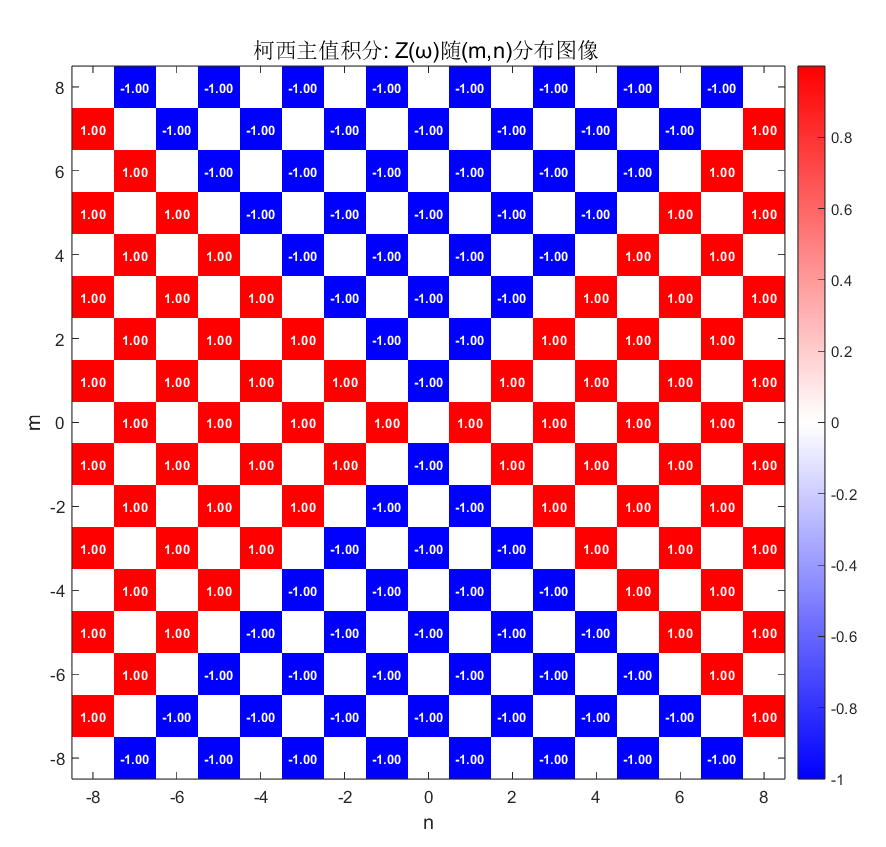
\includegraphics[width=0.6\textwidth]{Cauchy主值积分.png}
  \caption{临界频率下阻抗的数值验证($C=1\mathrm{F},L=1\mathrm{H}$)}
  \label{fig:Chauchy}
\end{figure}

\subsection{零阻抗的应用前景}

临界频率下奇偶性相同节点间阻抗为零的现象，在射频工程与传感技术中具有重要的应用价值。

\begin{enumerate}
    \item \textbf{零损耗射频信号传输}：传统微波传输线受导体损耗和介质损耗的制约，而临界频率下的 $LC$ 网格提供了一条无损信号路径\textsuperscript{\cite{444}}。通过选择奇偶性相同的节点对，信号可在理论上无耗地到达目标节点。该特性可应用于片上无线能量传输、可重构功率分配网络以及高效率射频前端的设计，显著降低系统功耗。
    
    \item \textbf{超灵敏传感与探测}：零阻抗节点对外部扰动极度敏感——若在该节点接入传感元件（如可变电容），其微小变化将打破零阻抗条件，导致阻抗发生剧烈跳变。这种突变可被高灵敏度检测，从而实现微弱物理/化学信号的放大机制，适用于生物分子检测、温度/压力传感以及网格缺陷定位等场景。
\end{enumerate}

此外，该现象为拓扑电路的室温实现提供了新思路：零阻抗路径对元件容差不敏感，可用于设计高鲁棒性的微波器件，并为高阶拓扑绝缘体的电路模拟奠定基础。


\subsection{其他频率的讨论}

对于 $\alpha \neq 1$ 的一般情况，积分(\ref{eq:I_mn_definition})的解析处理更为复杂，需引入椭圆积分或留数定理等数值方法，
对$m,n$在不同区域的讨论过于困难。限于笔者的数学能力，难以进行更进一步的推导。


\section{结论}

本文采用离散Fourier变换作为统一的分析工具，系统研究了两类具有平移对称性的
二维无穷网格电路的输运性质，分别针对纯电阻网络和电感-电容（$LC$）网络建立了从
基尔霍夫定律到等效响应函数的完整理论框架。主要结论如下：
 
\begin{enumerate}
    \item \textbf{纯电阻网格的等效电阻}：通过将实空间的差分方程变换至频域，
    获得了电势的闭合积分解，进而导出任意两点间等效电阻的二维积分表达式
    (\ref{eq:R_integral})。为进一步克服二维奇异积分在数值计算中的不便，
    本文利用变量代换与留数定理，将积分精确转化为快速收敛的双重级数(\ref{eq:R_series})
    。该级数各项以 $2^{-4k}$ 的速率衰减，显著提升了计算效率，且退化为平凡情形
    （$m=n=0$）时自动给出 $R_{00}=0$，验证了公式的自洽性。

    \item \textbf{一维二聚化$LC$传输线的谐振行为}：针对胞内、胞间电容非对称
    的二聚化$LC$链，建立了节点电压的转移矩阵方程，系统分析了三种特征频率下的
    谐振模式。特别地，当 $\omega = \dfrac{1}{\sqrt{L(C_1+C_2)}}$ 时，$A$、$B$ 两子
    格完全退耦合，$B$ 子格电压可独立置零而不影响 $A$ 子格的电压分布，呈现选择
    性接地效应；当 $\omega = \dfrac{1}{\sqrt{LC_1}}$ 时，系统展现出依赖电容比 $C_1/C_2$
     的丰富相行为，包括实根振荡（$C_1>2C_2$）、临界衰减（$C_1=2C_2$）以及复根衰
     减振荡（$C_1<2C_2$），并给出了各情形下电压分布的闭合解析表达式。

    \item \textbf{二维$LC$网格在临界频率的特殊阻抗行为}：对于横向电容、
    纵向电感构成的二维$LC$网格，推导了任意两点间阻抗的频域积分表达
    式(\ref{eq:Z_integral_2D})。在临界频率
     $\omega_0 = \dfrac{1}{\sqrt{LC}}$（即 $\alpha=1$）处，
     通过半角变换将二维积分化为菱形区域上的可分离变量积分，并利用区域对称性求得：
    \[
    \tilde Z(\omega_0) =
    \begin{dcases}
        -\ii\sqrt{\dfrac{L}{C}}\,\sgn(m-n)\,\sgn(m+n),
        & m \not\equiv n \pmod{2},\\[6pt]
        0, & \text{其他情况}.
    \end{dcases}
    \]
    该结果表明：当且仅当两节点横纵坐标奇偶性相异时，
    阻抗为纯虚数；当奇偶性相同时，
    阻抗严格为零。这一发现揭示了临界频率下网格中非局域
    的完全透射与完全阻断交替出现的奇特拓扑输运现象。
    数值计算的Cauchy主值积分（图\ref{fig:Chauchy}）
    与解析结果完全一致，验证了推导的正确性。

    \item \textbf{方法论的普适性}：纯电阻网格的椭圆型算子与$LC$网格的双曲型算子虽物理本质迥异，但Fourier变换均能将其统一处理为频域代数方程。差异仅在于后续积分的化简策略——电阻问题依赖级数展开，而$LC$临界问题则可通过变量替换实现分离变量精确求解。这一对比表明，离散Fourier变换是处理离散平移对称系统的一般性方法，而具体积分技巧则需根据算子类型灵活选择。
\end{enumerate}

综上所述，本文为二维无穷网格电路提供了一套从积分解到可计算级数或闭合表达式的完整理论方案，所有结果均经过自洽性检验与数值验证。研究不仅丰富了离散格林函数在电路理论中的应用，也为拓扑电路、超材料传输线等领域的进一步探索提供了可扩展的数学工具。


\begin{thebibliography}{99}

\bibitem{shu2014}
舒幼生，胡望雨，陈秉乾.
物理学难题集萃. 上册[M].
合肥：中国科学技术大学出版社，2014: 611-616.

\bibitem{cserti2000}
Cserti J.
Application of the lattice Green's function for calculating the resistance of an infinite network of resistors[J].
\textit{American Journal of Physics}, 2000, 68(10): 896-906.

\bibitem{english2026}
English L~Q, Halchenko A, Palmero F.
Topologically protected spatially localized modes: An easy experimental realization of the Su–Schrieffer–Heeger model[J].
\textit{Physica B: Condensed Matter}, 2026, 734: 418616.

\bibitem{444}
Sahin H.
Topoelectrical circuit theory and realizations of topological, non-linear, and non-Hermitian phenomena[D].
Singapore: National University of Singapore, 2024.


\end{thebibliography}



% ==================== 附录 ====================
\clearpage
\appendix
\section{$I$的计算过程}\label{A}
记
\begin{equation}
  J(a)=\dfrac{1}{2}\int_{-\pi}^\pi\cos au\cos^ku\di u
\end{equation}

令$z=\e{\ii u}$，则有
\begin{equation}
  \di z=\ii\e{\ii u}\di u=\ii z\di u
\end{equation}
\begin{align*}
  J(a)&=\dfrac{1}{2\ii}\oint_{|z|\leqslant1}\dfrac{z^a+z^{-a}}{2}\dfrac{\left(z+z^{-1}\right)^k}{2^k}z^{-1}\di z\\
  &=\dfrac{1}{2^{k+2}\ii}\oint_{|z|\leqslant1}\dfrac{\left(z^{2a}+1\right)}{z^{a+k+1}}\left(z^2+1\right)^k\di z\\
  &=\dfrac{1}{2^{k+2}\ii}\oint_{|z|\leqslant1}\sum_{t=0}^{k}\binom{k}{t}z^{2t}\dfrac{\left(z^{2a}+1\right)}{z^{a+k+1}}\di z\\
  &=\dfrac{-\ii}{2^{k+2}}\sum_{t=0}^{k}\binom{k}{t}\oint_{|z|\leqslant1}\left(\dfrac{1}{z^{k+a+1-2t}}+\dfrac{1}{z^{k-a+1-2t}}\right)\di z\\
\end{align*}

利用留数定理，只需算被积函数洛朗展开$z^{-1}$系数
\begin{equation}
  J(a)=\dfrac{\pi}{2^{k+1}}\left[\binom{k}{\frac{k+a}{2}}+\binom{k}{\frac{k-a}{2}}\right]=\dfrac{\pi}{2^k}\dfrac{k!}{\left(\frac{k+a}{2}\right)!\left(\frac{k-a}{2}\right)!}
\end{equation}

考虑$J(a)$关于$k$的取值，
\begin{equation}
  J(a)=
  \begin{dcases}
    \dfrac{\pi}{2^k}\dfrac{k!}{\left(\frac{k+a}{2}\right)!\left(\frac{k-a}{2}\right)!},&|a|\leqslant k,k\equiv a\,(\text{mod}2)\\
    0,&\text{other}.
  \end{dcases}
\end{equation}

同理于$J(a)$，
\begin{equation}
  J(b)=
  \begin{dcases}
    \dfrac{\pi}{2^k}\dfrac{k!}{\left(\frac{k+b}{2}\right)!\left(\frac{k-b}{2}\right)!},&|b|\leqslant k,k\equiv b\,(\text{mod}2)\\
    0,&\text{other}.
  \end{dcases}
\end{equation}

考虑$J(a)J(b)$：
\begin{enumerate}
  \item $a,b$必然同奇偶；
  \item 三角不等式$|a|\geqslant|b|$。
\end{enumerate}
故$I_2$的求和中只有$k=a+2p,p=0,1,2,\cdots$对求和有贡献。所以，$I_2$中关于$k$的求和换成对$p$的求和
\begin{align}
  I_2=\sum_{p=0}^{\infty}\dfrac{2\pi^2}{2^{2a+4p}}\dfrac{(a+2p)!}{p!(a+p)!}\dfrac{(a+2p)!}{(\frac{a-b}{2}+p)!(\frac{a+b}{2}+p)!}
\end{align}

注意$a,b$的定义式，并将$p$替换回$k$，又有
\begin{equation}
  I_2=\dfrac{2\pi^2}{2^{2(m+n)}}\sum_{k=0}^{\infty}\dfrac{1}{2^{4k}}\dfrac{(m+n+2k)!}{k!(m+k)!(n+k)!(m+n+k)!}
\end{equation}

结合$I_1,I_2$的表达式，得出积分$I$的级数为
\begin{equation}
  I=I_1-I_2=2\pi^2\sum_{k=0}^{\infty}\dfrac{1}{2^{4k}}\left[\left(\dfrac{(2k)!}{k!k!}\right)^2-\dfrac{(m+n+2k)!^2}{2^{2(m+n)}k!(m+k)!(n+k)!(m+n+k)!}\right]
\end{equation}








\section{Dirichlet核积分的计算}\label{D}

此积分在 $\alpha=1$ 的精确解中使用。定义
\begin{equation}
  S_K\equiv\int_{-\pi}^{\pi}\dfrac{\sin(K\theta)}{\sin\theta}\,\di\theta.
\end{equation}

$K$ 为奇数：令 $K=2M+1$（$M\ge 0$）。由 Dirichlet 核：
\begin{equation}
    \frac{\sin((2M+1)\theta)}{\sin\theta} = 1 + 2\sum_{j=1}^{M}\cos(2j\theta).
\end{equation}
每一项 $\cos(2j\theta)$（$j\ge 1$）在 $[-\pi,\pi]$ 上积分为零，仅常数项贡献 $2\pi$。故 $S_{2M+1} = 2\pi$。

$K$ 为偶数：令 $K=2M$（$M\ge 1$）：
\begin{equation}
    \dfrac{\sin(2M\theta)}{\sin\theta} = 2\sum_{j=1}^{M}\cos[(2j-1)\theta].
\end{equation}
每一项频率均为奇数，积分为零。故 $S_{2M} = 0$。

综上：
\begin{equation}
    \boxed{
    S_K =
    \begin{cases}
        2\pi, & K \equiv 1 \pmod{2},\\
        0, & K \equiv 0 \pmod{2}.
    \end{cases}
    }
    \label{eq:C1}
\end{equation}



\end{document}